\section*{1. Coordinate system}

a) Define \textbf{zenith}, \textbf{nadir}, the \textbf{celestial north} and \textbf{south poles}, and the
\textbf{meridian line}. Draw the meridian plane of an observer, including the position of the observer 
(*), the zenith (Z), the meridian line, and the north (N) and south (S) poles.\\
\\
\begin{itemize}
    \item \textbf{zenith}: Point which is directly over the observer on a celestial sphere
    \item \textbf{nadir}: Point which is directly under the observer on a celestial sphere
    \item \textbf{celestial north pole}: Northern point of the Earth's rotation axis
    \item \textbf{celestial south pole}: Southern point of the Earth's rotation axis
    \item \textbf{meridian line}: Great circle that passes through the celestial poles
\end{itemize}

\noindent\makebox[\textwidth]{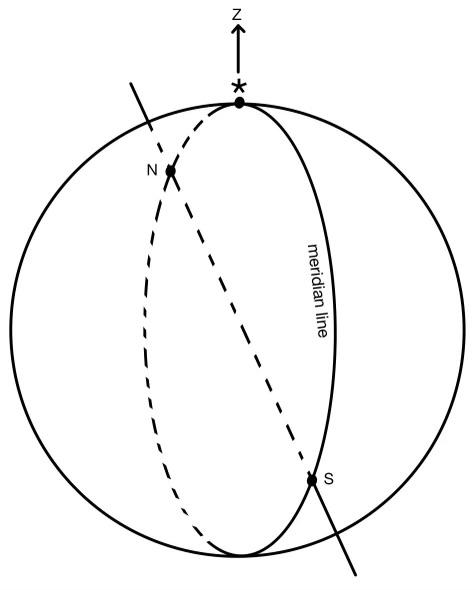
\includegraphics[scale=0.35]{meridian_plane.jpeg}}
\noindent
b) An observer located in the Earth's Northern Hemisphere observers the top and bottom culminations of
circumpolar star. Measuring $h_i = 20 \degree \: 22' \: 32.4''$ ; $A_i = 180 \degree$ for the hight and
azimuth of the bottom culmination and $h_s = 50 \degree \: 23' \: 08.2''$ ; $A_s = 180 \degree$ for the
upper culmination. What is the observer's latitude $\phi$?\\
\\
First of all we convert the measured hights:
\begin{equation*}
    \begin{split}
        h_i &= 20 \degree \: 22' \: 32.4''\\
            &= 20 \degree + \frac{22 \degree}{60} + \frac{32.4 \degree}{3600}\\
            &\approx 20 \degree + 0.36666667 \degree + 0.009 \degree\\
            &= 20.37566667 \degree\\
        h_s &= 50 \degree \: 23' \: 08.2''\\
            &= 50 \degree + \frac{23 \degree}{60} + \frac{08.2 \degree}{3600}\\
            &\approx 50 \degree + 0.38333333 \degree + 0.00227778\degree\\
            &= 50.3856111 \degree\\
    \end{split}
\end{equation*}
Next I assume that the azimuth is for both measurments $0 \degree$ and not $180 \degree$, because if the
observer is on the Northern Hemisphere and looking south there is no way the star would be circumpolar
for him at the angles $50 \degree$ and $20 \degree$. With that in mind we can calculate the altitude of
Polaris to determine the observer's latitude since the star circles around Polaris and its altitude will 
be equal to the observer's latitude. We calculate Polaris' altitude by determining the radius of the 
circle drawn around him on the celestial sphere and adding the lower culmination to the radius.
\begin{equation*}
    \begin{split}
        \phi &= \frac{h_s - h_i}{2} + h_i\\
             &= \frac{50.3856111 \degree - 20.37566667 \degree}{2} + 20.37566667 \degree\\
             &= \frac{30.00994443 \degree}{2} + 20.37566667 \degree\\
             &= 15.004972215 \degree + 20.37566667 \degree\\
             &= 35.380638885 \degree\\
    \end{split}
\end{equation*}
The observer's latitude is $35.380638885 \degree$ north.\\
\\
\noindent
c) Determine the maximum height in the sky that the globular cluster $\omega$Cen (declination 
$\delta = -47 \degree \: 29'$) reaches when observed from the Inter-American Observatory of Cerro Tololo,
Chile (latitude $\phi = -30 \degree \: 10' \: 20.9''$)\\
\\
The Inter-American Observatory has a latitude of $-30 \degree \: 10' \: 20.9''$, which means that the 
south pole of the celestial sphere is seen from that point of view at an angle of 
$30 \degree \: 10' \: 20.9''$. The declanation of $\omega$Cen is $-47 \degree \: 29'$, which means that
the angle between it and the celestial equator is $47 \degree \: 29'$ and since the celestial south pole
is at $-90 \degree$, $\omega$Cen is $90 \degree - 47 \degree \: 29'$ or $42 \degree \: 31'$ away from the
south pole. So at the upper culmination $\omega$Cen will be seen highest at 
$42 \degree \: 31' + 30 \degree \: 10' \: 20.9''$ or $72 \degree \: 41' \: 20.9''$ from the Inter-American 
Observatory with an azimuth of $180 \degree$.
